\documentclass[10pt,a4paper]{article}
\usepackage{latexsym}
\pagestyle{headings}
\usepackage[latin1]{inputenc}
\usepackage[dvips]{graphicx}
\usepackage[dvips]{color}


\usepackage{amsmath}
\usepackage{amsfonts}
\usepackage{amstext}


% 
\usepackage{listings}
\lstset{ frame=Ltb,
     framerule=0pt,
     aboveskip=0.5cm,
     framextopmargin=3pt,
     framexbottommargin=3pt,
     framexleftmargin=0.5cm,
     framesep=0pt,
     rulesep=.4pt,
     backgroundcolor=\color{gray97},
     rulesepcolor=\color{black},
     %
     stringstyle=\ttfamily,
     showstringspaces = false,
     basicstyle=\small\ttfamily,
     commentstyle=\color{gray45},
     keywordstyle=\bfseries,
     %
     numbers=left,
     numbersep=15pt,
     numberstyle=\tiny,
     numberfirstline = false,
     breaklines=true,
   }

%

\usepackage[activeacute,english,spanish]{babel}
\usepackage{geometry}
\usepackage{pstricks}

\usepackage{fancyhdr}
\pagestyle{fancy}
\usepackage{fancybox}

\usepackage{lastpage}
\addtolength{\headwidth}{\marginparwidth}
\addtolength{\headwidth}{\marginparsep}
\fancypagestyle{plain}% Para la primera página
{%
         \fancyhead[l]{}
         \fancyhead[r]{\bfseries}
         \fancyhead[c]{}
         \renewcommand{\headrulewidth}{0.5pt}
         \fancyfoot[l]{\scriptsize \textit{Armando. B. VERA}\normalsize}
         \fancyfoot[c]{}
         \fancyfoot[r]{\scriptsize\thepage/\pageref{LastPage} \normalsize}
         \renewcommand{\footrulewidth}{0.5pt}
}
% Para el resto de páginas
\lhead{}
\chead{}
\rhead{\bfseries La clase CFecha Desde Adentro}
\renewcommand{\headrulewidth}{0.3pt}
\lfoot{\scriptsize \textit{Prof.: Armando. B. VERA}}
\cfoot{}
\rfoot{\scriptsize \thepage/\pageref{LastPage} \normalsize}
\renewcommand{\footrulewidth}{0.3pt}
%\geometry{left=3.5cm, right=2.3cm, top=3.5cm, bottom=2.5cm}
\geometry{right=2.2cm,bottom=2.5cm}
\usepackage{tikz}
%\setlength{\fboxrule}{1 pt} \setlength{\fboxsep}{8pt}
\setlength{\shadowsize}{2pt}
\usepackage{url}
\usepackage[all]{xy}




\usepackage{amsmath}
\usepackage{amsfonts}
\usepackage{amssymb}





\author{prof. en  Matem\'atica e Inform\'atica Armando B. VERA}
\title{La Clase CFecha}
\begin{document}
\begin{abstract}
\textsf{Esta clase se dise\~n\'o y construy\'o para servir como medio de aprendizaje. Muchas de las t\'ecnicas uitilizadas son b\'asicas pero son las primeras que se aprenden. Un ejemplo de ellos es la utilizaci\'on del if-else en lugar del operador ?: que es m\'as compacto.}
\end{abstract}
\section*{Dise\~no}
   
   \begin{center}
    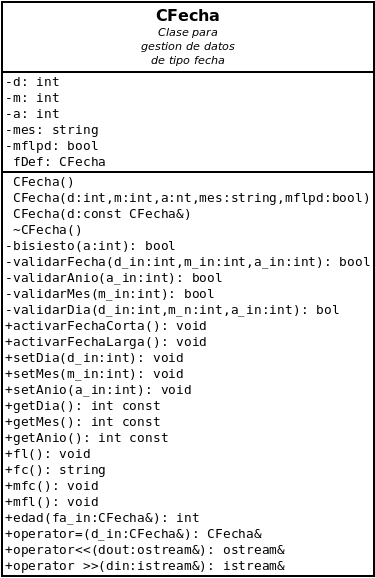
\includegraphics[scale=0.7]{CFecha.png}
   \end{center}
   
\section*{Utilizaci\'on}
Para poder utilizar la clase \texttt{CFecha}, debe incluir el archvo de cabecera \texttt{CFecha.h}. Hay varias formas en que puede hacerse esto, la misma se explica en la secci\'on de instalaci\'on.

Vamos a crear una aplicaci\'on de prueba de la clase al que llamaremos \texttt{testClaseCFecha.cpp} y lo guardaremos en el mismo directorio CFECHA

 \color{orange}
 \begin{verbatim}
 // testClaseCFecha.cpp
 #include <iostream>
 #include "CFecha.h"
 
 using namespace std;
 
 int main(){
    CFecha miCumple; // miCumple se inicializa con los valores definido en fDef
    miCumple=(24,08,1968); // Asignamos una fecha a miCumple
    ...
 } 
 \end{verbatim}
 \color{black}

Con la instrucci\'on \texttt{CFecha miCumple} se define una variable de tipo CFecha, una instancia de esa clase. Se reserva memoria para alojar un objeto de esta clase y se inicializa con los valores por defecto (Definida en la variable est\'atica \texttt{fDef}).  \texttt{miCumple} es un objeto de la clase CFecha y posee toda la funcionalidad que le hayamos podido proporcionar a dicha clase.

Si deseamos asignar una fecha diferente podemos utilizar cualquiera de las formas siguientes: \\ \texttt{miCumple=(24,08,1968)} o bien \texttt{miCumple=CFecha(24,08,1968)}, en este \'ultimo caso se crea una nueva variable de tipo \texttt{CFecha} y se asignan cada atributo uno a uno utilizando el operador de asignaci\'on (=) sobrecargado. Una vez copiada, la variable reci\'en creada se destruye.

Es importante definir una fecha por defecto en las aplicaciones para, en caso de inicializarse un objeto de la clase con una fecha inv\'alida, pueda esta incializarse con los valores por defecto. Esta variable de tipo fecha y perteneciente a la misma clase es est\'atica y salta la comprobaci\'on por lo que se debe tener sumo cuidado al inicializarlas. El siguiente c\'odigo muestra c\'omo hacerlo.

\color{orange}
\begin{verbatim}
// testClaseCFecha.cpp
# include "CFecha.h" // Depende como lo hayas instalado
...
CFecha CFecha::fDef(1,1,1974);
...
int main() {
   ...
}
\end{verbatim}
\color{black}



Es posible utilizar la fecha del sistema para asignar de forma autom\'atica la fecha actual a una variable de tipo CFecha. Utilizando en c\'odigo siguiente podemos obtener el efecto buscado.

\color{orange}
\begin{verbatim}
\\testClaseCFecha.cpp
...
#include <ctime>
...
int main() {
   ...
   struct tm *fh;
   time_t segundos;
   time(&segundos);
   fh=localtime(&segundos);
   int dh=(int)fh->tm_mday
   int mh=(int)fh->tm_mon +1; // tm en time.h
   int ah=(int)fh->tm_year+1900;

   CFecha hoy(dh,mh,ah);
   ...
}
\end{verbatim}
\color{black}

La aplicaci\'on archivo fuente es \texttt{testClaseCFecha.cpp} posee ahora una variable global llamada \texttt{hoy} igual a la fecha del sistema y puede ser muy \'util para calcular la edad de una persona a partir de la fecha de nacimiento.

\subsection*{M\'etodos de actualizaci\'on}

La clase posee los siguientes m\'etodos (funciones) que permiten actualizar los datos de un objeto de la clase en forma particular. Los prototipos de estas funciones son: \\
\color{orange}
\begin{verbatim}
   bool setDia(int dia_in), 
   bool setMes(int mes_in) y 
   bool setAnio(int a_in)
\end{verbatim}
\color{black}




\section*{Una Introducci\'on al dise\~no de CFecha}
La clase utiliza tres variables de tipo \texttt{int}, en su secci\'on privada, para representar d\'ia, mes y a\~no. Adem\'as utiliza un objeto de tipo \texttt{string} para la representaci\'on del mes en forma de cadena y una variable de tipo \textit{bool} para activar y desativar las formas en que la fecha es mostrada por medio de un objeto del flujo de salida estandar ostream.

Po \'ultimo utiliza una variable de tipo CFecha est\'atica para utilizarla como fecha por defecto. Al ser est\'atica se debe de tener cuidado de no introducir una fecha incorrecta ya que no se efect\'ua la comprobaci\'on del mismo. En la siguiente secci\'on se muestra una parte del archivo de cabecera \textit{CFecha.h}

\color{orange}
\begin{verbatim}
/* ********** CFecha.h *************** */
/* *************************************
PROGRAMACION ORIENTADA A OBJETOS CON C++
		prof. Armando B. VERA
************************************** */
#ifndef _CFECHA_H_
#define _CFECHA_H_

#include <iostream>
#include <ostream>
#include <istream>
#include <string>
#include <ctime>
#include <limits>

class CFecha{
   private:
      int d;
      int m;
      int a;
      std::string mes;
      bool mflpd; // true: muestra fecha larga por defecto	

      bool bisiesto(int a_in);
      bool validaFecha(int d_in, int m_in, int a_in);
      bool validaAnio(int a_in);
      bool validaMes(int m_in);
      bool validaDia(int d_in, int m_in, int a_in);
	
      static CFecha fDef; // Fecha por defecto
   ...
}	
\end{verbatim}
\color{black}

Adem\'as de los cinco atributos descritos anteriormente observamos declarado cuatro funciones de tipo \textit{bool} cuya func\'on es la de validar o comprobar si las fechas son correctas antes de ser asignados a una variable (objeto) del tipo \texttt{CFecha}, queda excluida de esta comprobaci\'on la variable est\'atica \texttt{fDef}. Las definiciones de estas funciones figuran en el archvio \textit{CFecha.cpp} que se estudiar\'a m\'as adelante.

\subsection*{Interfaz}

Se utiliza un constructor con valores por defecto. Como es l\'ogico, esta debe estar en su secci\'on p\'ublica. Iremos mostrando fragmentos del archvo de cabecera \textit{CFecha.h} conforme vamos explicando.

\color{orange}
\begin{verbatim}
\end{verbatim}
\color{black}


\color{orange}
\begin{verbatim}

class CFecha{
...
public:
CFecha(int d_in=0, int m_in=0, int a_in=0, std::string mes="", bool mflpd=false);
static void set_fDef(int d_in, int m_in, int a_in, std::string mes, bool mflpd); 
CFecha(const CFecha& f);
~CFecha();
	...
}
\end{verbatim}
\color{black}

En la primera l\'inea de su parte p\'ublica figura el constructor. Se utilica un constructor con valores por defecto que, como puede notarse, no son fechas v\'alidas. Esto se hace de esta forma para asignarse la fecha por defecto en caso de que el usuario pretenda introducir una fecha inv\'alida o no introduzca ninguna fecha.

El constructor nos permite introducir fechas como \texttt{CFecha miCumple(24,08,68)} o bien, con la instrucci\'on \texttt{CFecha miCumple=(24,08,68)}. 

Tambie\'en podemos definir variables (objetos) de tipo fecha as\'i \texttt{CFecha miFecha}. En este caso, se asignan los valores por defecto, pero como nos son fechas v\'alidas, no pasa la comprobaci\'on y se asigna la fecha por defecto, es decir la fecha definida en \texttt{fDef} 

el atributo de tipo \textit{bool} \texttt{mflpd} (Mostrar fecha larga por defecto) se utiliza para determinar c\'omo se mostrar\'a la fecha cuando se utilice el operador ``$<<$'' de inserci\'on en el flujo de salida ostream. Si este atributo es \textit{true} se mostrar\'a   ``$25$ de Febrero de $2015$'' cuando se utilice el \texttt{cout}, y si es falso, se mostrar\'a ``25 de Feb de 2015''.

Los m\'etodos de actualizaci\'on deben pasar por un filtro para determinar si son valores v\'alidos. Si no los son, se debe proporcionar alg\'un mecanismo que permita cambiar los valores incorrectos o bien considerar la posibilidad de no efectuar la actualizaci\'on, pero eviando un mensaje informando de tal situaci\'on.

\subsection*{El m\'etodo \textit{bool setDia(int d\_in)}}

La definici\'on de este m\'etodo es el siguiente:

\color{orange}
\begin{verbatim}
...

bool CFecha::setDia(int d_in){
   if(validaDia(d_in, m, a) && validaMes(m) && validaAnio(a)){
      d=d_in;
      return true;
   } else {
     throw errorFecha(); // Tratamiento de error
     return false;
   }
}
...

\end{verbatim}
\color{black}

Este m\'etodo es invocado desde un objeto del tipo \texttt{CFecha} con valores ya asignados a sus par\'ametros, por lo tanto debe comprobar si el d\'ia que se pasa por par\'ametro puede ser asignado a ese objeto fecha. Supongamos que la fecha es ``25 de febrero de 2015'' y queremos cambiar a la fecha ``29 de febrero de 2015''. En este caso, nuestra clase debe impedir tal asignaci\'on ya que el d\'ia 29 para el mes de febrero de ese a\~no no existe. La opci\'on m\'as sensata es no hacer el cambio y enviar o mostrar un aviso sobre la causa de la no asignaci\'on. La funci\'on (o el m\'etodo si si lo prefiere) \textit{bool validaDia(int d\_in)} producir\'a un valor falso haciendo que el if no se cumpla. Es importante hacer notar que \textit{bool validaDia(intd\_in)} llama a la funci\'on \textit{bool bisiesto(int a\_in)}

\subsubsection*{utilizaci\'on}

Vamos a suponer la situaci\'on planteada en lo p\'arrafos anteriores. Definimos un objeto fecha al que llamaremos \textbf{diaD}, es decir, \texttt{CFecha diaD=CFecha(25,02,2015)}. Queremos que \textbf{diaD} en lugar de  $25$ sea $29$. Llamamos al m\'etodo para hacer dicho cambio

\texttt{diaD.setDia(29);}

Tras haber sido llamado el m\'etodo de actualizaci\'on, nuestra fecha seguir\'a con la fecha antigua. El encargdo de darle el tratamiento adecuado es \texttt{throw errorFecha()}. Aqu\'i hay que hacer notar que es fundamental que el dise\~no de la clase debe contemplar todas esas posibilidades y darle la posiblidad de un tratamiento adecuado. 

\subsection*{Tratamiento del error en la clase}
Cuando se tiene la responsabilidad de dise\~nar una clase, si la idea es hacerlo robusta, funcional, simple y usable hay que verse como un usuario. 




\end{document}